\documentclass[letterpaper]{article}
\usepackage{aaai}
\usepackage{times}
\usepackage{helvet}
\usepackage{courier}
\usepackage{graphicx}
\usepackage{enumerate}
\frenchspacing
\setlength{\pdfpagewidth}{8.5in}
\setlength{\pdfpageheight}{11in}
\pdfinfo{
/Title (Insert Your Title Here)
/Author (Put All Your Authors Here, Separated by Commas)}
\setcounter{secnumdepth}{0}  
 \begin{document}
% The file aaai.sty is the style file for AAAI Press 
% proceedings, working notes, and technical reports.
%
\title{Handwritten Font Generator \\ Based on StyleGAN}
\author{Chengruidong Zhang, Haoran Xi}
\maketitle

\section{Problem Statement}
A font consists of a set of character images sharing the same style. Because each character has a fixed skeleton, we may be able to extract the style information from limited character images and apply it to all characters. This means that a new font can be created with very few character images as input, and everyone can create his / her handwritten font without writing all the characters.

\begin{center}
    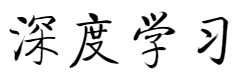
\includegraphics[]{proposal-fig-qiti.png}
    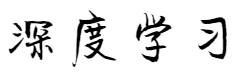
\includegraphics[]{proposal-fig-jinglei.png}

    Figure 1. Same characters in different fonts.\\The second font is more uneven and compact.
\end{center}


\section{Related Works}
\subsection{Image Style Transfer Using CNN}
It is an algorithm that can separate and recombine the image content and style of natural images. A Convolutional Neural Network is trained to extract high level image information and produce new images of high perceptual quality that combine the content of an arbitrary photograph with the appearance of specified artworks. This work proves the feasibility of using CNN for image style transfer.
\subsection{StyleGAN}
StyleGAN is a GAN architecture with a style-based generator that receives additional inputs to adjust the style. It leads to an automatically learned, unsupervised separation of high-level attributes and stochastic variation in the generated images, and it enables intuitive, scale-specific control of the synthesis.

\subsection{SKFont: skeleton-driven Korean font generator}
With a limited sample of Korean characters, this research investigates the topic of font synthesis using an end-to-end conditional deep adversarial network. Only 114 samples are required for the SKFont model to generate the remaining characters in the same font style. This is accomplished in three steps.

\begin{enumerate}
\item generate complete target font characters by observing 114 target characters
\item extract the structures of the synthesized characters obtained from the first step
\item transfer the style of the target font onto these learned structures
\end{enumerate}
This approach resolves flaws such as blurriness, breakage, and a lack of delicate shape and style delivery.


\subsection{Word Level Font-to-Font Image Translation}
They propose a network that can convert any printed text image's font style from its existing font to the desired font. Since the network is trained end-to-end for the complete word images, it eliminates the necessary pre-processing steps, like character segmentation. To learn the one-to-many mapping function, they apply conditional setting. It also aids in the consistency of the final images after concatenating the target font's generated image patches. The majority of previous image translation research has been done on square pictures. This is the first architecture of its sort that can accommodate images of varied widths.



\section{Dataset}
The dataset includes $32 \times 32$ images of common characters converted from different font files. System fonts such as Brush Script MT and Segoe Script can be used at the beginning. More handwritten fonts will be collected if necessary. We plan to start with English characters and numbers, and then introduce Chinese characters.

\section{Model}
We plan to build a Generative Adversarial Network, which consists of a 5-layer Style-based generator and a 3-layer conditional discriminator. The input and output are both $32 \times 32$ single-channel (black and white) images.
\\
On each training epoch, images of two different fonts are fed into the model, providing skeleton and style information, respectively.
\begin{center}
    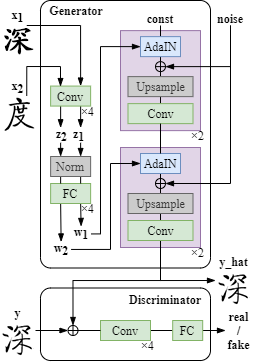
\includegraphics[scale=0.7]{plan-fig-model.png}

    Figure 2. General structure of\\our generator and discriminator. 
\end{center}
Denote an image of character $c$ and font $f$ by $I[c,f]$. For each time, the generator takes a pair of images $(I_1=I[c_i,f_0], I_2=I[c_j,f_k])$ and outputs an image $I_o$ with skeleton of $I_1$ and style of $I_2$. The discriminator differs the output from the groundtruth - image $I[c_i,f_k]$. Font $f_0$ should have clear skeletons, and can be the same whenever training or testing.

\section{Anticipated Outcomes}
To be specific, the generator is expected to (1) separate the structure and style information of a image and (2) apply the style information to another image. The discriminator should be able to tell whether a pair of images describe the same character and belong to the same font.
\\
Therefore, a well-trained generator can generate images of any character in the style of any input image $I_2$. If we input a handwritten character image repeatly with all common characters $I[c_i,f_0]$, we'll get a new handwritten font.

\section{Challanges and Concerns}
\begin{itemize}
    \item The typical StyleGAN extracts style information using fully-connected networks, which may not be able to seperate the style and skeleton of character images well. We may need a pre-trained skeleton extractor rather than roughly putting images into the generator.
    \item The skeleton provider, $I[c_i,f_0]$, also plays the role of identifier. If our generator have the ability to remember the skeleton shape of all characters, we can replace the input $I_1$ of one-hot character codes.
    \item Notice that fonts are stored in the form of vector graphs of quadratic Bezier curves. The final model should include a image trace module to output vector graphs.
\end{itemize}

\section{Reference}
smallskip \noindent
Leon, A. G., Alexander, S. E., and Matthias, B. 2016. Image Style Transfer Using Convolutional Neural Networks. \textit{CVPR}, pp. 2414-2423.

\smallskip \noindent
Tero, K., Samuli, L., and Timo, A. 2019. A Style-Based Generator Architecture for Generative Adversarial Networks. \textit{CVPR}, abs/1812.04948.

\smallskip \noindent
Ko, D. H., Hassan, A. U., Suk, J., \& Choi, J. 2021. SKFont: skeleton-driven Korean font generator with conditional deep adversarial networks. \textit{International Journal on Document Analysis and Recognition (IJDAR)}, 1-13.

\smallskip \noindent
Bhunia, A. K., Bhunia, A. K., Banerjee, P., Konwer, A., Bhowmick, A., Roy, P. P., \& Pal, U. 2018. Word level font-to-font image translation using convolutional recurrent generative adversarial networks. \textit{ICPR} (pp. 3645-3650).



\bibliography{proposal-reference.bib}
\bibliographystyle{aaai}
\end{document}